% Pipeline figure for Methods — keep in sync with § The Iteration Loop
% Requires only: \usepackage{tikz}  (no positioning / arrows.meta libraries)
\begin{figure}[t]
  \centering
  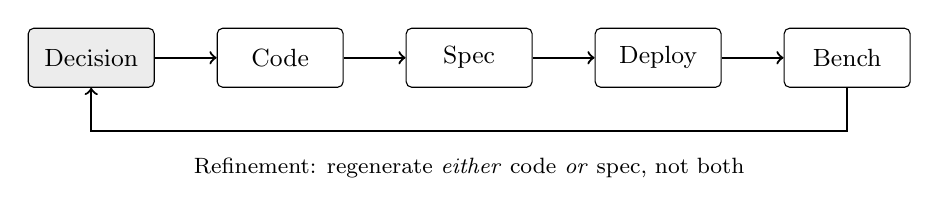
\begin{tikzpicture}[
    font=\small,
    stage/.style={
      draw, rounded corners=2pt, align=center,
      minimum width=1.6cm, minimum height=0.75cm,
      inner sep=2pt
    },
    decision/.style={stage, fill=gray!15},
    arr/.style={->, thick}
  ]
    \node[decision] (dec) at (0,0) {Decision};
    \node[stage] (code) at (2.4,0) {Code};
    \node[stage] (spec) at (4.8,0) {Spec};
    \node[stage] (dep) at (7.2,0) {Deploy};
    \node[stage] (bench) at (9.6,0) {Bench};

    \draw[arr] (dec) -- (code);
    \draw[arr] (code) -- (spec);
    \draw[arr] (spec) -- (dep);
    \draw[arr] (dep) -- (bench);

    \draw[arr] (bench.south) -- ++(0,-0.55) -| (dec.south);

    \node[font=\footnotesize, anchor=north] at (4.8,-1.15) {%
      Refinement: regenerate \emph{either} code \emph{or} spec, not both};
  \end{tikzpicture}
  \caption{Pipeline stages of one iteration.  After a successful bench, feedback
    conditions the next decision.  On the baseline the decision LLM is skipped
    and both code and specification are generated; on refinement only one of
    those two is regenerated.  After a code or specification failure the next
    lever is forced (decision LLM skipped).}
  \label{fig:pipeline}
\end{figure}
